\documentclass{article}
\usepackage[margin=1in]{geometry}  % set the margins to 1in on all sides
\usepackage{graphicx}              % to include figures
\usepackage{epstopdf}
\usepackage{amsmath}               % great math stuff
\usepackage{amsfonts}              % for blackboard bold, etc
\usepackage{amsthm}                % better theorem environments
\usepackage{amssymb}
\usepackage[english]{babel}
\usepackage[utf8]{inputenc}
\usepackage{fancyhdr}
\usepackage{tikz}
\usepackage{lipsum,array,amsmath}
\usetikzlibrary{positioning,automata}
\usetikzlibrary{arrows.meta}
\usepackage{pgfplots}
\usepackage{amsmath}
\DeclareMathOperator*{\argmax}{argmax}
\DeclareMathOperator*{\argmin}{argmin}
\usepackage{hyperref}
\usepackage{caption}
\usepackage{subcaption}
\usepackage{float}
\usepackage[ruled,vlined]{algorithm2e}

\DeclareUnicodeCharacter{00D7}{x}
\pagestyle{fancy}
\fancyhf{}

\lhead{CMPUT-615: Project Report}
\rfoot{Page \thepage}
\lfoot{\scriptsize{}}


\begin{document}


% =================== Header ====================
\begin{center}
{CMPUT-615: Project Report}  \\ 
\Large{\textbf{3D Model Based Tracking}}  \\
\vspace{.1in}
\begin{table}[H]
\center
\begin{tabular}{clc}
\begin{tabular}[c]{@{}c@{}}Islam Ali\\Department of Computing Science\\University of Alberta\\iaali@ualberta.ca \end{tabular} & \hspace{3cm} & \begin{tabular}[c]{@{}c@{}}Junaid Ahmad\\Department of Computing Science\\University of Alberta\\ jahmad@ualberta.ca\end{tabular}
\end{tabular}
\end{table}
\end{center}
\vspace{5pt}
\hrule
\vspace{2pt}
\section*{Abstract}
Abstract Goes Here ... 
\vspace{5pt}
\hrule
\vspace{10pt}
% ============================================================
\section{Problem Definition}
Object tracking is one of the main corner stones in a wide spectrum of robotics-related applications. This is true for both regular 2D tracking, and 3D object tracking which allow robots to perform more tasks. In this project, we study the problem of 3D Model-Based Tracking, which is tracking 3D object with the knowledge of its 3D structure in prior. We study one of the main systems that most of modern trackers are based on, which is RAPiD \cite{harris1990rapid}. We focus on the study of the system structure and how the task can be achieved, pinpointing main problems with RAPiD tracking and proposing solutions when applicable. The system will be tested on synthetic data as a starting point with the purpose of having it tested with real-world data in the near future. The main performance metric is the tracking accuracy for the time being, with plans to focus on memory and complexity aspects as the system evolves in the future.
% ============================================================
\section{Literature Review}
\subsection{Taxonomy of 3D Tracking Systems}
\subsection{Performance Evaluation}
% ============================================================
\section{System Design}
As mentioned earlier, the system is based on the famous 3D Model Based Real-time tracking developed by Harris et. al.\cite{harris1990rapid}. The following is a block diagram of the full system illustrating the different components and their interaction with each other. 
\begin{figure}[H]
\centering
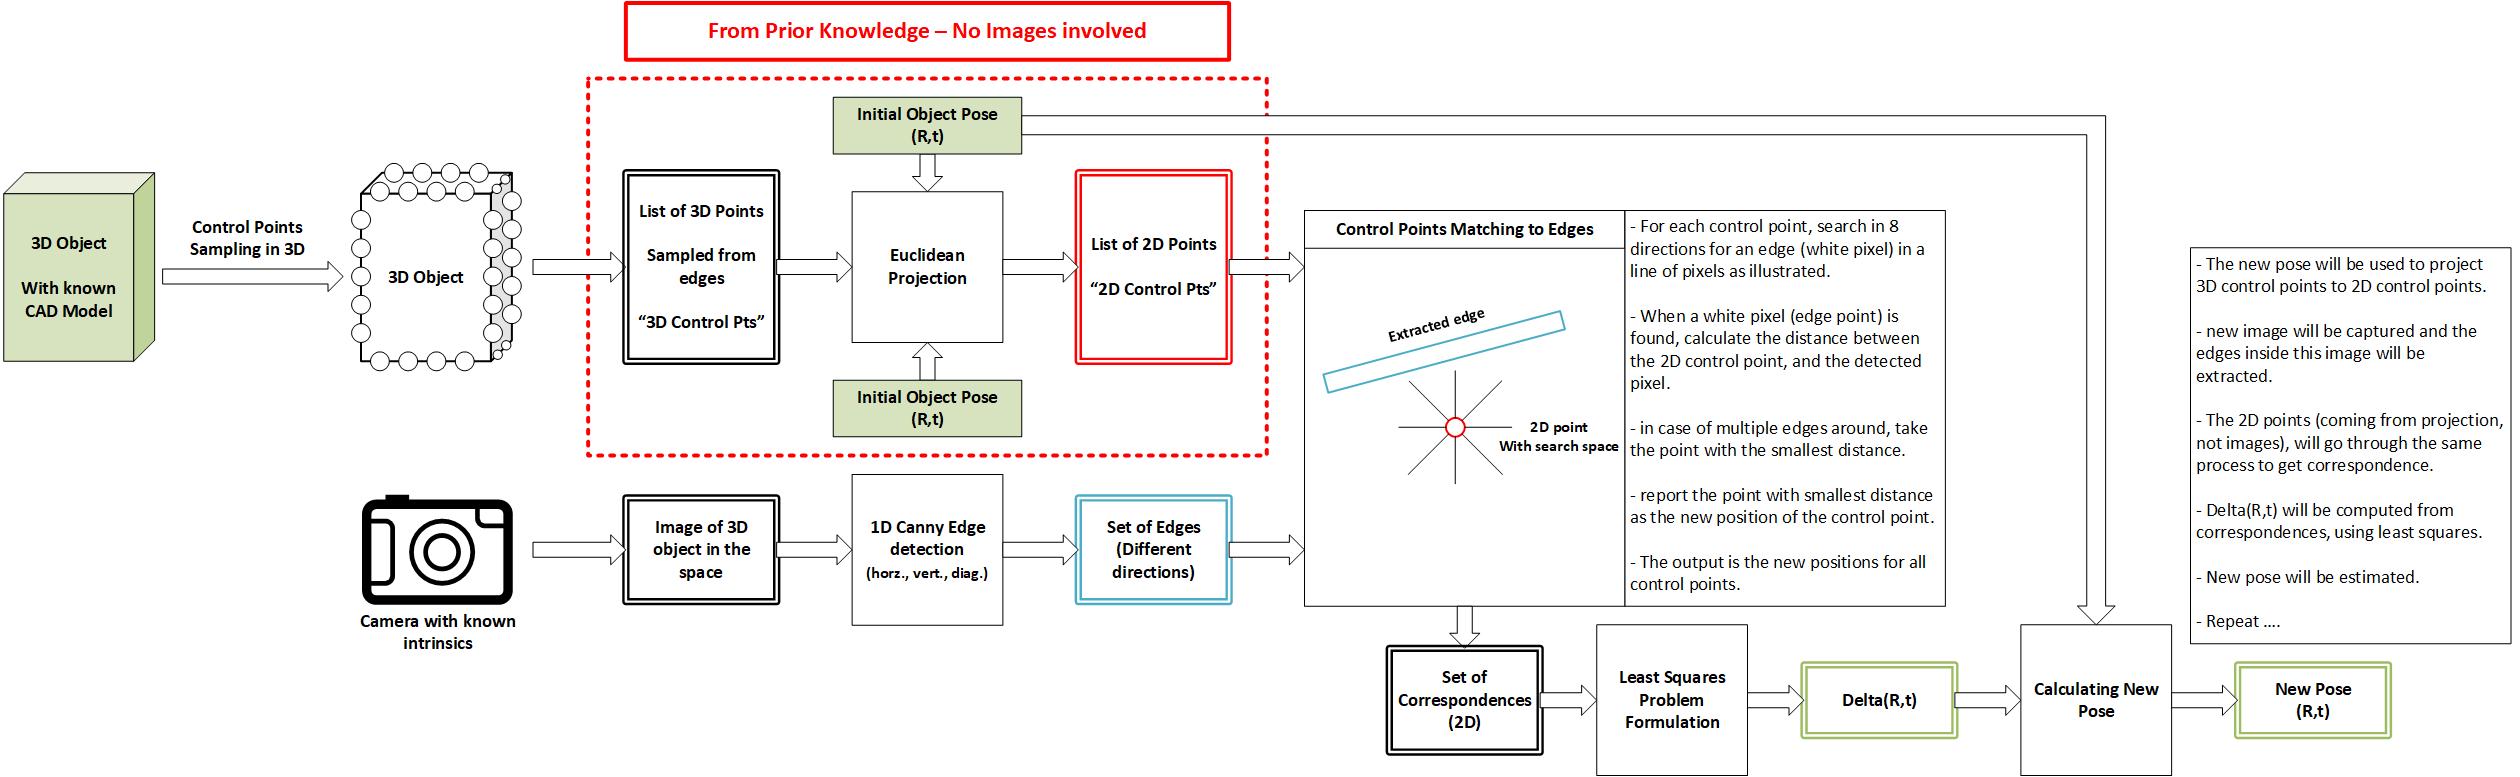
\includegraphics[width=\textwidth]{RAPiD_BlockDiagram.png}
\caption{Full System Block Diagram}
\end{figure}
From an abstract point of view, the idea for RAPiD\cite{harris1990rapid} is based on tracking high-contrast edges which we call control edges. However, edges are not dealt with directly but through a sampling step where these edges are samples to a number of points along each edge. These points are then called control points and they act as the basis for next steps. Next, we should have an estimate of the 3D object pose, which at the beginning can come from calibration, and as we progress can have the value for the previous estimated pose at the previous time step. The process is mainly project the 3D control points onto the image using the object pose and camera calibration parameters. Then search for the closest edge to each one of these points. After finding the corresponding 2D points, we construct a least squares equation in order to infer the values for the motion in terms of translation and rotation. The pose of the object is then updated based on the inferred motion values. In the rest of this section, we provide the detailed design of the system as well as the mathematical representation of the motion screw and how it was obtained. We also show how the least squares formulation in our case was a bit different from the original least squares format provided in \cite{harris1990rapid} due to the fact that the camera in our case does not align with neither the object frame nor with the world frame. \\
From a detailed point of view, the system goes through two different states which are:
\begin{enumerate}
\item Bootstrapping
\item Motion estimation loop
\end{enumerate}

\subsection{Bootstrapping}
Bootstrapping is considered the system initialization phase and has the objective of having an initial state for the following items:
\begin{enumerate}
\item Camera calibration parameters (both intrinsic and extrinsic).
\item 3D model for the object to be tracked with proper representation.
\item 6D pose of the object w.r.t. the world coordinate frame.
\end{enumerate}
Due to having a synthetic data set, we needed to extract these parameters from the blender model. In real-world setup, the system should undergo formal calibration procedure, formal measurements of pose of camera in the world frame, and proper measurement of both the object dimensions and complete pose.

\subsection{Motion Estimation Loop}
One the system is initialized and the aforementioned information are available and are accurate enough, the system tries to estimate the pose of the 3D object in the world coordinate frame using the following algorithm:
\begin{algorithm}[H]
\SetAlgoLined
\KwResult{6D object pose}
 Determine the initial 6D pose of the object\;
 Perform camera calibration (intrinsic and extrinsic)\;
 3D control points = sampling (high contrast 3D edges) \;
 \While{Image Sequence Not End}{
  2D control points = Projection of 3D points using pose info and camera calibration\;
  sobel image = extract image edges using Sobel operator\;
	
	\For{Each control point}{
		l = length from 2D projected point to closest edge\;
		corresponding 2D point = point with shortest length to edge\;
		Add corresponding point to correspondence vector\;
	}  
  Filter correspondences and keep only strong ones\;
  $\Delta p$ = least squares on correspondences \;
  Update object pose: $p = p+ \Delta p$\;
 }
 \caption{RAPiD 3D Model-Based Tracking}
\end{algorithm}

\subsubsection{Control Points Projection}
Having a set of 3D control points sampled from high contrast object edges, we are able to project these 3D points onto 2D image plane with the knowledge of the camera calibration matrices and the object pose in the world coordinate system. The projection is applied to the homogeneous form of the 3D points and takes the following form:
\begin{equation}
\begin{bmatrix}
x \\ y \\ w 
\end{bmatrix} = [K][Rt]_{camera} [Rt]_{object} \begin{bmatrix}
X \\ Y \\ Z \\ 1
\end{bmatrix}
\end{equation}
Then the 2D projection of each point is retained by normalizing the result as follows:
\begin{equation}
\begin{bmatrix}
u \\ v
\end{bmatrix} = \begin{bmatrix}
x/w \\ y/w
\end{bmatrix}
\end{equation}
\subsubsection{Edge Detection and Extraction}
Extraction of image edges is crucial as we need to find correspondences for projected points in each image. These correspondences will allow us to deduce the motion screw of the 3D object. A wide range of methods are available for edge detection and extraction. In our case, we tried both Canny edge detector \cite{canny1986computational} and Sobel-Feldman operator \cite{Sobel1990AnI3}. In our case and due to the lighting conditions of the synthetic scene, Sobel-Feldman was selected as our edge detector of choice. \\
Sobel-Feldman operator\cite{Sobel1990AnI3} is a gradient based edge detection method that computes the first order derivative separately for each of the image dimensions $x$ and $y$. The derivative is calculated by performing convolution of the image with a two 3x3 kernels, one for each dimension, which computes approximation for the gradient. This gradient is able to highlight high frequencies inside images which are usually produced by edges. The Sobel-Feldman kernels are as follows:
\begin{equation}
kernel_x = \begin{bmatrix}
-1 & 0 & +1 \\ -2 & 0 & +2 \\ -1 & 0 & +1
\end{bmatrix} \;\;\;\;\;\;\;\;
kernel_y = \begin{bmatrix}
+1 & +2 & +1 \\
0 & 0 & 0 \\
-1 & -2 & -1 
\end{bmatrix}
\end{equation}
To suppress weak edges and emphasize strong ones, image thresholding is applied to the result of the Sobel-Feldman convolution and the threshold value is tuned to be $I_{threshold} = 127$ which remove some of the shadows and emphasize real images. 
\subsubsection{Corresponding Edges Extraction}
The original RAPiD \cite{harris1990rapid} assumes that, if the motion done by the object being tracked is small enough, the control edge (projected), and the image edge (extracted from image) should be parallel to each other. Therefore, a 1D search can be done in the direction perpendicular to the control edge from the control point for image intensities. Once an edge pixel is detected, it is declared as the correspondence for this control point. For simplicity, and to cover multiple motion profiles of the object, the search is done in 8 directions around each control point which are: horizontal, vertical, and diagonal. 
\subsubsection{Correspondences Filtering}
In order to avoid having noise in the estimation in the least squares step, correspondences must be filtered to ensure consistency. The simplest method is to filter based on the euclidean distance to nearest edge. In the current setup, this threshold is set to be $d_{threshold} =50$, meaning that, if the closest edge is $50pixels$ or more far away from the point, the corresponding point is considered to be at infinity, and this control point is then excluded from the vector of correspondences sent to least squares. Other filtering can be done such as using RANSAC\cite{fischler1981random} algorithm to ensure consistency over correspondences before deducing motion screw based on them.
\subsubsection{Least Squares Formulation}
This step is concerned about finding the motion increment that the 3D object made in the 3D world. It is represented by 6DoFs which are 3D translation and 3D rotation. The derivation for this least squares formula will differ from the derivation mentioned in \cite{harris1990rapid} \cite{lepetit2005monocular} due to the difference in assumptions, as such, they assume that the relation between the object and the camera is just translation denoted as $T$ and they assume that there is no rotation involved. However, in our case, we do have rotation and translation between the camera frame and the world frame and therefore between the object frame and the camera frame. We believed that the formula derived in this section is more generic to a wider spectrum of situations. \\
Given a 3D point $P$ in the world coordinate frame, and a camera that has the relation to the world frame governed by the rotation matrix $R$ and the translation vector $T$. Point $P$ can be represented in the camera coordinate system as:
\begin{equation}
M = RP+T
\end{equation}
Assume that the object performed a small motion that is represented by a change of position $\Delta t$ and a change in rotation $\delta r$. The point projection in the camera frame after this small motion is given by:
\begin{equation}
M^{'} = R(\Delta r.P+\delta t )+ T
\end{equation}
Harris\cite{harris1990rapid} assumed that the rotation $\Delta r$ can be linearized to be:
\begin{equation}
\Delta r = I+\delta \Omega
\end{equation}
Where $\delta \Omega$ is a skew symmetric matrix of the 3D rotation vector, and is given by:
\begin{equation}
\delta \Omega = \begin{bmatrix}
0 & -\omega_z & \Omega_y \\
\Omega_z & 0 & -\Omega_x \\
-\Omega_y & \Omega_x & 0
\end{bmatrix}
\end{equation}
Providing the formula $M^{'}$ in terms of $M$ is given by:
\begin{equation}
M^{'} = R.P + R. \delta\Omega.P+R.\delta t + T
\end{equation}
Given the formula: $M=RP+T$, we can re-write the above equation as:
\begin{equation}
M^{'} = M + R. \delta\Omega P + R \delta t
\end{equation}
To represent this equation in terms of the image projection, both $M$ and $M^{'}$ should be projected to the image plane using the intrinsic camera matrix:
\begin{equation}
m = KM \;\;\;\;\;\;\;\; m^{'} = k M^{'}
\end{equation}
However, the inputs to our system is image correspondences $m$ and $m^{'}$, therefore, these input points needs to be normalized by the intrinsic camera matrix.
\begin{equation}
\begin{bmatrix}u \\ v \end{bmatrix} = K^{-1}m = M 
\;\;\;\;\;\;\;\; 
\begin{bmatrix}u^{'} \\ v^{'} \end{bmatrix} = K^{-1}m^{'} = M^{'}
\end{equation}
Expanding the above equations and omitting all nonlinear terms, will result:
\begin{equation}
u^{'} = u + \frac{1}{T_z + P_z} (\delta t_x + \delta \Omega_y P_z - \delta \Omega_z P_y - u(\delta t_z+\delta \Omega_x P_y -\delta \Omega_y P_x))
\end{equation}
\begin{equation}
v^{'} = v + \frac{1}{T_z + P_z} (\delta t_y + \delta \Omega_z P_x - \delta \Omega_x P_z -v(\delta t_z+\delta \Omega_x P_y -\delta \Omega_y P_x) )
\end{equation}
Which can be re-written in the following matrix format:
\begin{equation}
\begin{bmatrix}
u^{'} - u \\ v^{'}-v
\end{bmatrix} = \begin{bmatrix}
-u P_y & P_z + u P_x & -P_y & 1 & 0 & -u \\
-P_z - v P_y & v P_x & P_x & 0 & 1 & -v
\end{bmatrix} \begin{bmatrix}
\delta \Omega_x \\
\delta \Omega_y \\
\delta \Omega_z \\
\delta t_x \\
\delta t_y \\
\delta t_z 
\end{bmatrix}
\end{equation}
Given that the distance between the projected 2d point and the corresponding 2d point is mainly a vector and is given by:
\begin{equation}
l = k^{-1}(m^{'} - m)
\end{equation}
The above matrix can be re-written to be:
\begin{equation}
l = W \delta p
\end{equation}
Which is a least squares formulation that can be solved alliteratively, or by the closed form given as:
\begin{equation}
\delta p = (W^{T} W)^{-1} W^{T} l
\end{equation}
The resulting motion screw $\delta p$ must be represented in the world frame, and this can be done by multiplication to the inverse of the rotation matrix between the camera and the world frame:
\begin{equation}
\delta p_{world} = R^{-1} \delta p
\end{equation}
By finding this quantity, we are able to update the object pose in the world frame successfully. 
\subsubsection{Object Pose Update}
After the transformation of the motion screw to the world coordinate system, we can update 3D control points by the following equation:
\begin{equation}
P_{new} = P_{old} + [[\delta \Omega]_{\times} |\delta t] P_{old}
\end{equation}
Where $[\delta \Omega]_{\times}$ is the skew symmetric matrix of the vector of rotation increment.
% ============================================================
\section{Results and Discussion}
\subsection{Experimental Setup}
For the sake of having full control over the environment, a synthetic scene was rendered using blender 2.8 that includes a cereal box-like object that does simple movements in the 3 axes, followed by rotation around the 3 axes, and finally performing composite motions that include both translation and rotation around one or multiple axes at a time. The sequence yielded 800 images with 9 high contrast edges visible during the whole sequence. The sequence was used for testing and evaluation of different system blocks. The objective is to also test the system against real video sequence in order to confirm the generalization of the solution and to pinpoint possible enhancements to the pipeline to allow it to be a suitable solution for real-world tasks.

\begin{figure}[H]
\centering
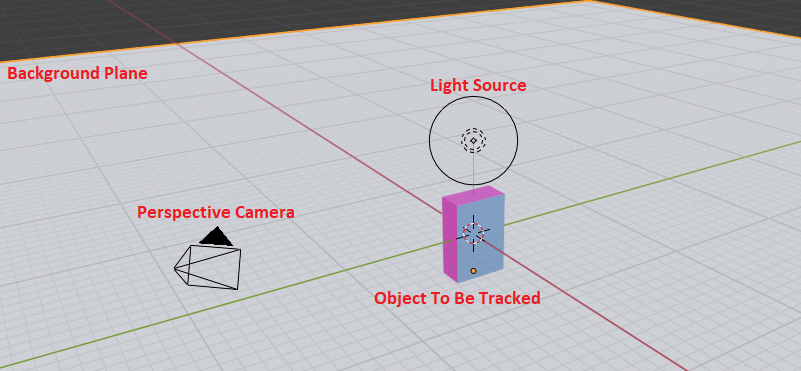
\includegraphics[width=\textwidth]{env_model.png}
\caption{Synthetic Environment Diagram Showing Its Components}
\end{figure}

\subsection{3D Model of Tracked Object}
The 3D model is a cereal box-like object with dimensions of 1 x 2 x 3 m located at the center of the world frame. The object vertexes are extracted from blender and was supplied to our code. The object is represented as a matrix of size 12x6, were each row represent an edge and each edge is represented by the two end points of this edge. The points locations are supplied in the world coordinate frame.  
\begin{figure}[ht]
\begin{subfigure}{.31\textwidth}
  \centering
  % include first image
  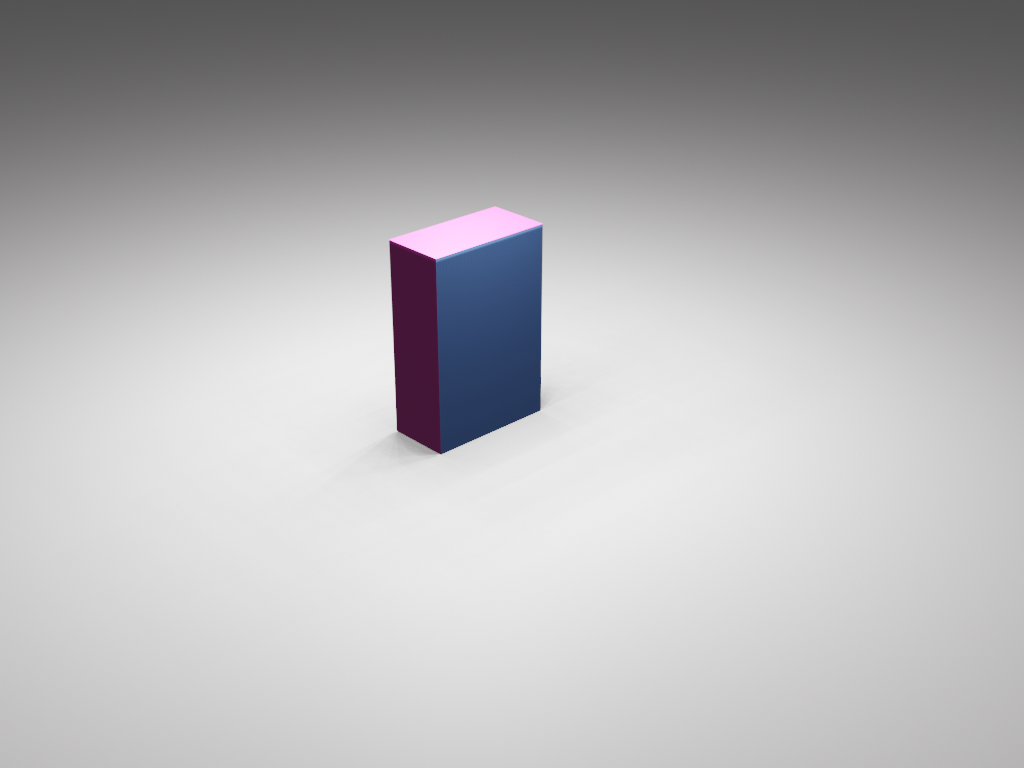
\includegraphics[width=.8\linewidth]{0001.png}  
  \caption{frame \# 1}
\end{subfigure}
\hfill
\begin{subfigure}{.31\textwidth}
  \centering
  % include second image
  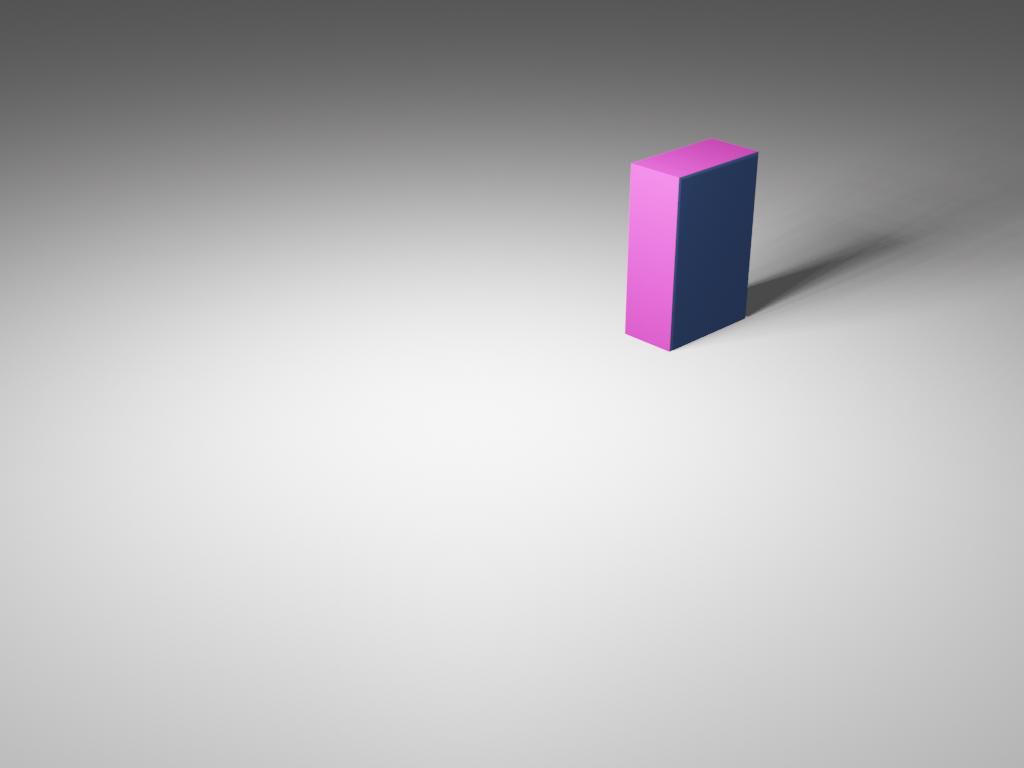
\includegraphics[width=.8\linewidth]{0100.png}  
  \caption{frame \# 100}
\end{subfigure}
\hfill
\begin{subfigure}{.31\textwidth}
  \centering
  % include second image
  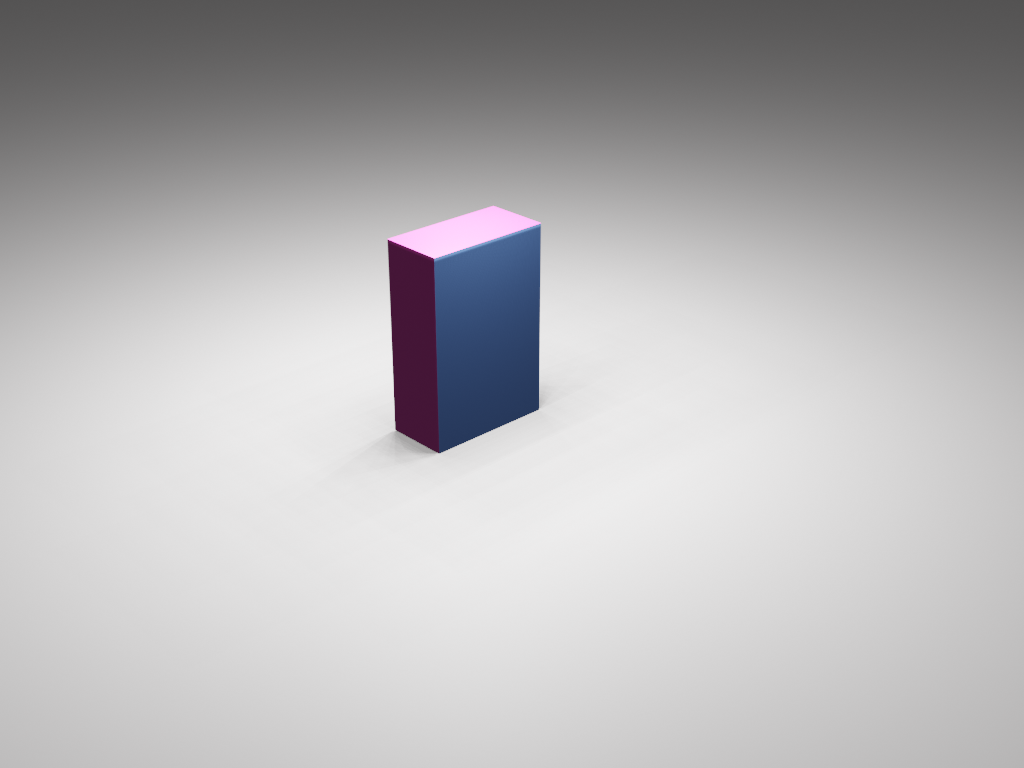
\includegraphics[width=.8\linewidth]{0200.png}  
  \caption{frame \# 200}
\end{subfigure} 
\\
\begin{subfigure}{.31\textwidth}
  \centering
  % include first image
  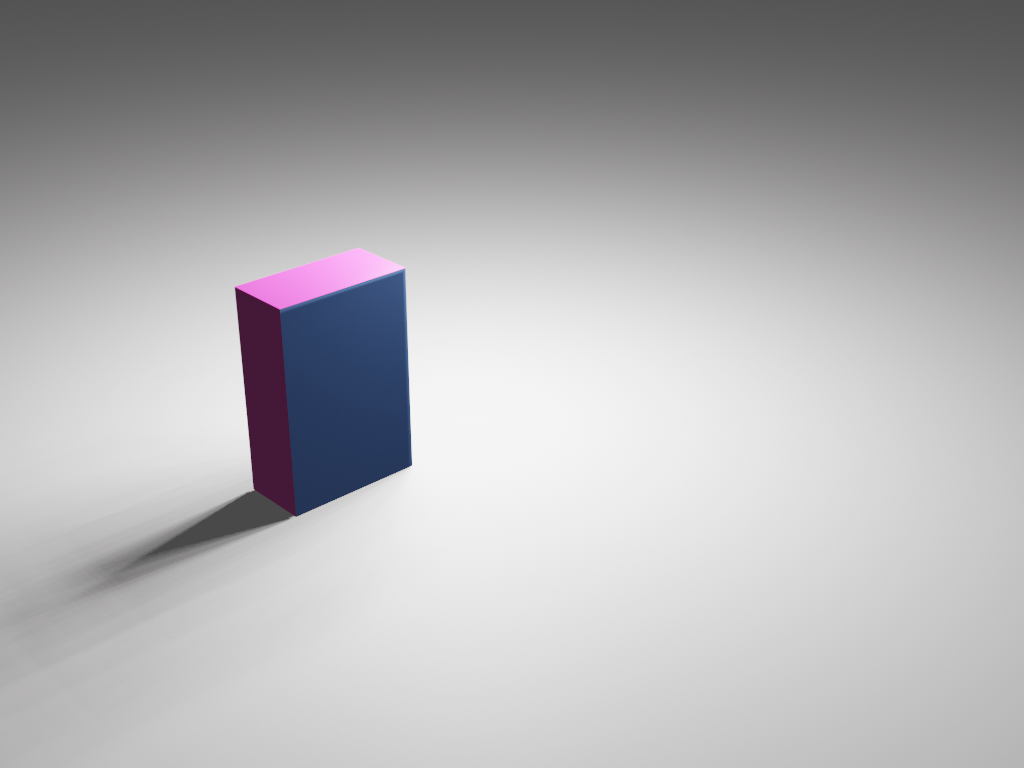
\includegraphics[width=.8\linewidth]{0300.png}  
  \caption{frame \# 300}
\end{subfigure}
\hfill
\begin{subfigure}{.31\textwidth}
  \centering
  % include second image
  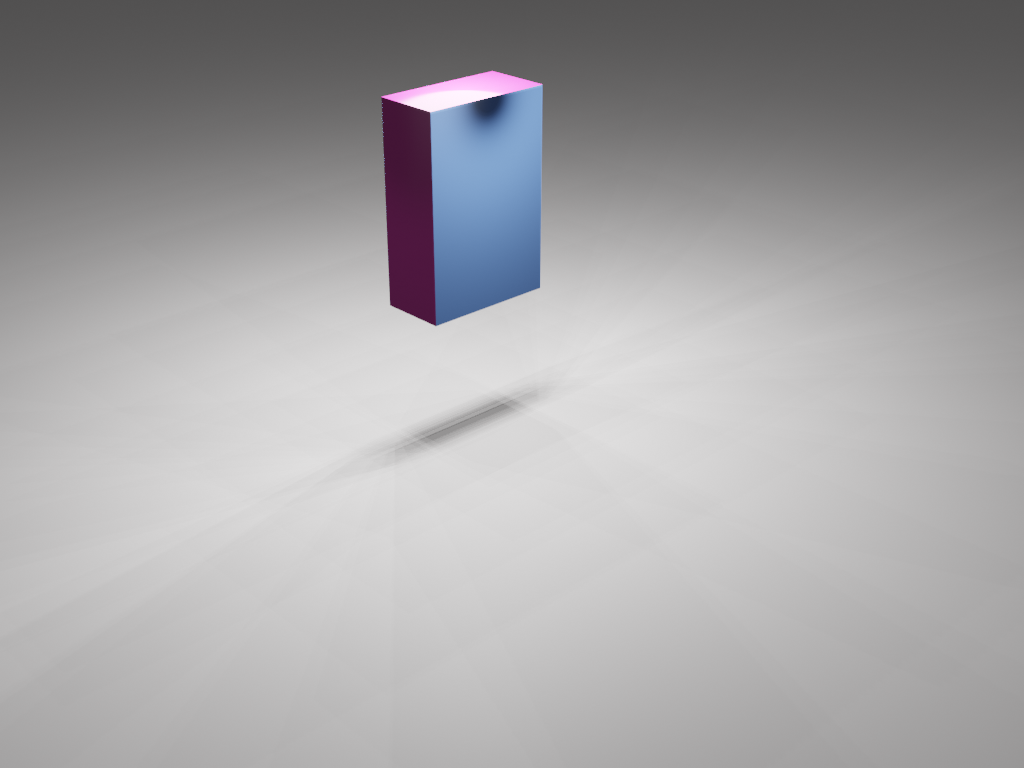
\includegraphics[width=.8\linewidth]{0400.png}  
  \caption{frame \# 400}
\end{subfigure}
\hfill
\begin{subfigure}{.31\textwidth}
  \centering
  % include second image
  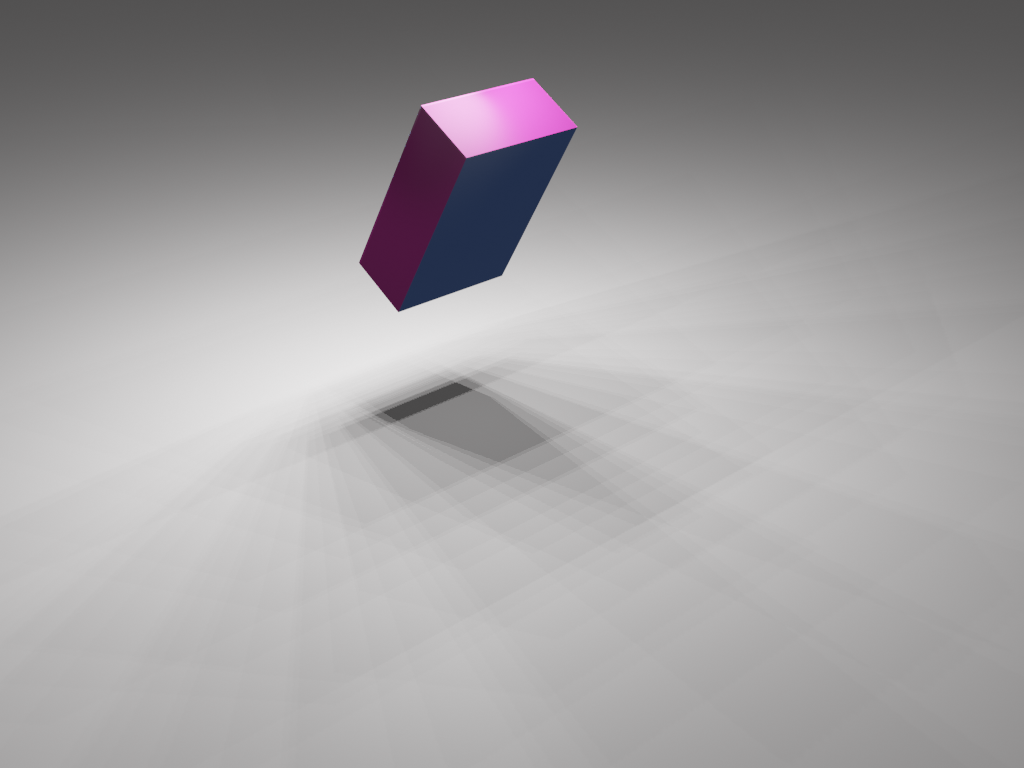
\includegraphics[width=.8\linewidth]{0500.png}  
  \caption{frame \# 500}
\end{subfigure} 
\\
\begin{subfigure}{.31\textwidth}
  \centering
  % include first image
  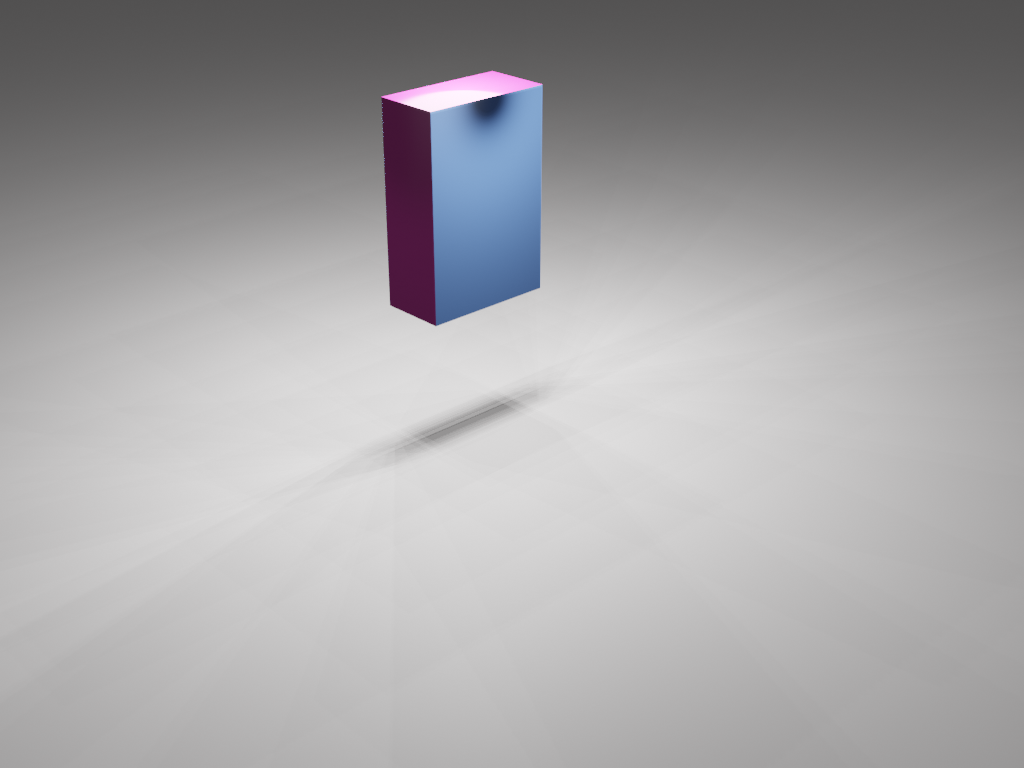
\includegraphics[width=.8\linewidth]{0600.png}  
  \caption{frame \# 600}
\end{subfigure}
\hfill
\begin{subfigure}{.31\textwidth}
  \centering
  % include second image
  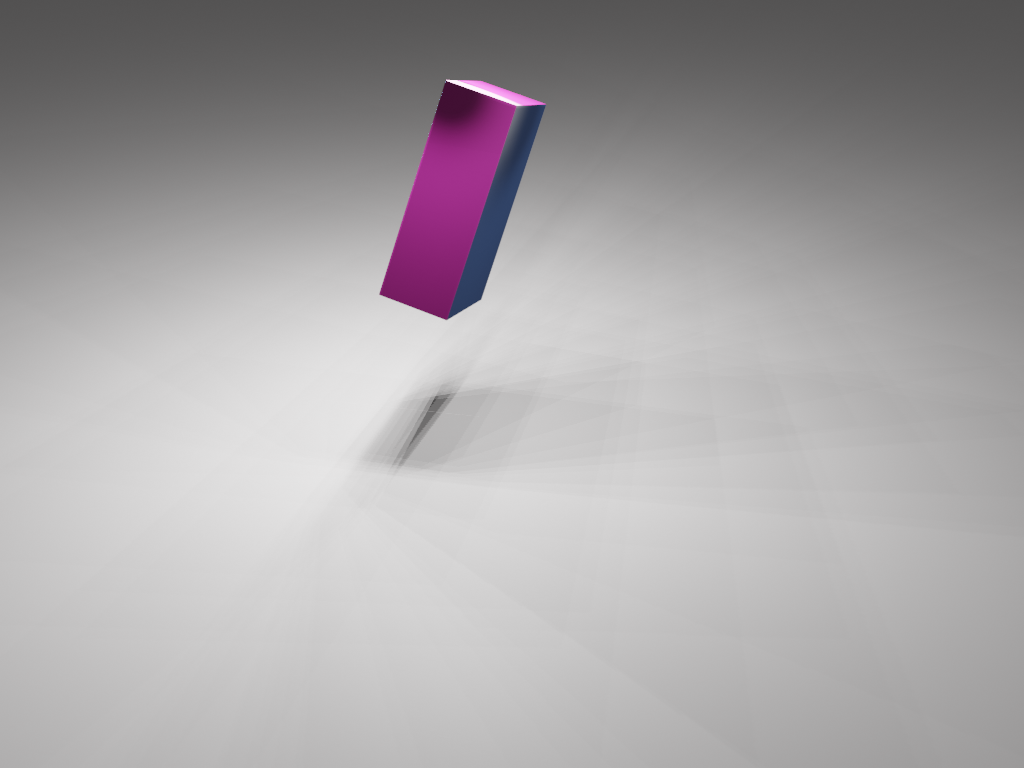
\includegraphics[width=.8\linewidth]{0700.png}  
  \caption{frame \# 700}
\end{subfigure}
\hfill
\begin{subfigure}{.31\textwidth}
  \centering
  % include second image
  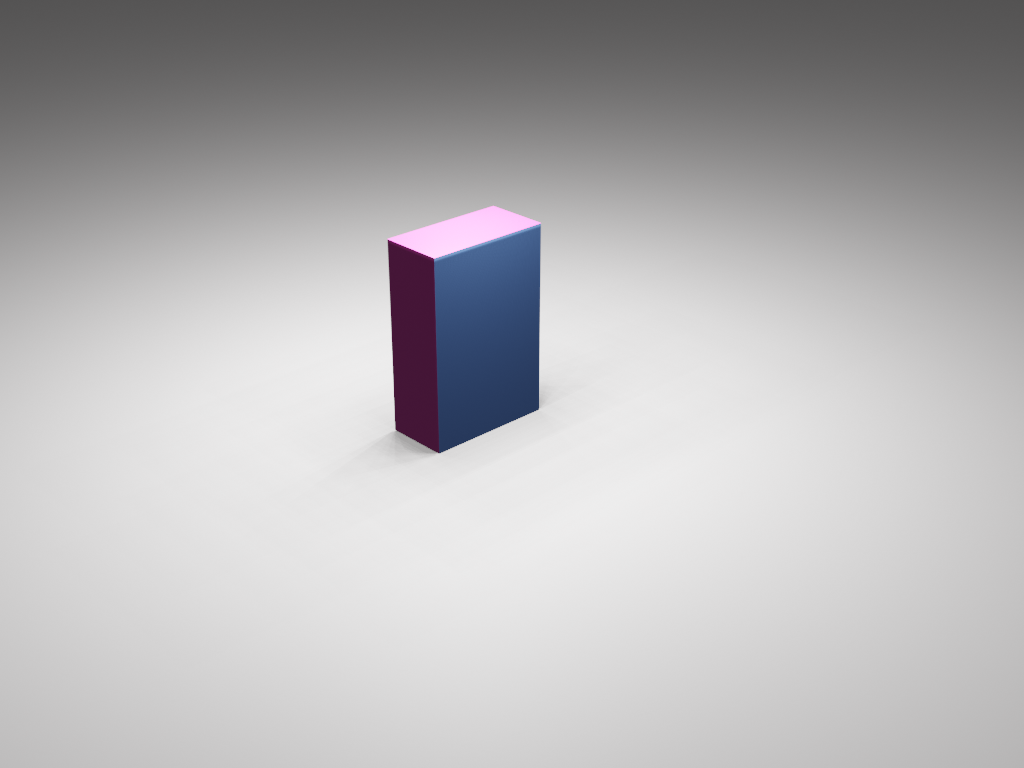
\includegraphics[width=.8\linewidth]{0800.png}  
  \caption{frame \# 800}
\end{subfigure} 
\caption{Samples Frames from the Synthetic Data Set}
\end{figure}

\subsection{Camera Calibration}
Due to having a synthetic data set, the camera calibration parameters are extracted from blender. The code was used to generate the full camera matrix (having intrinsic and extrinsic parameters), extrinsic alone, and intrinsic alone. The results were then plugged into our integrated system in a configuration file. The following is the extracted camera information from the blender model.
\begin{table}[H]
\centering
\begin{tabular}{|l|c|c|}
\hline
\textbf{Image Size}                       & 1024 x 768                   & Pixels  \\ \hline
\textbf{Focal Length}                     & (1422.2, 1422.2)             & mm      \\ \hline
\textbf{Principle Point}                  & (512, 384)                   & Pixels  \\ \hline
\textbf{Distortion Factor}                & (0, 0)                       & \%      \\ \hline
\textbf{Camera Translation (World Frame)} & (28.3589, -24.9258, 16.9583) & m       \\ \hline
\textbf{Camera Rotation (World Frame)}    & (63.5593, 0, 46.6919)        & Degrees \\ \hline
\end{tabular}
\caption{Synthetic Camera Calibration Parameters}
\end{table}

\subsection{System Results}
\subsection{Discussion}
% ============================================================
\section{Future Work}
Section
% ============================================================
\section*{Conclusion}
% ============================================================
\newpage
\pagenumbering{Roman}
\bibliographystyle{ieeetr}
\bibliography{journal09}
 
\end{document}